\documentclass{article}

\usepackage{graphicx}
\usepackage{tikz}
\usepackage{tikzsymbols}
\usetikzlibrary{calc,patterns,shapes.geometric}
\pagestyle{empty}
\usepackage[margin=0pt]{geometry}
\geometry{papersize={14in,12in}}

\def\centerarc[#1](#2)(#3:#4:#5){\draw[#1] ($(#2)+({#5*cos(#3)},{#5*sin(#3)})$) arc (#3:#4:#5);}

\begin{document}
	\begin{figure}
		\centering
		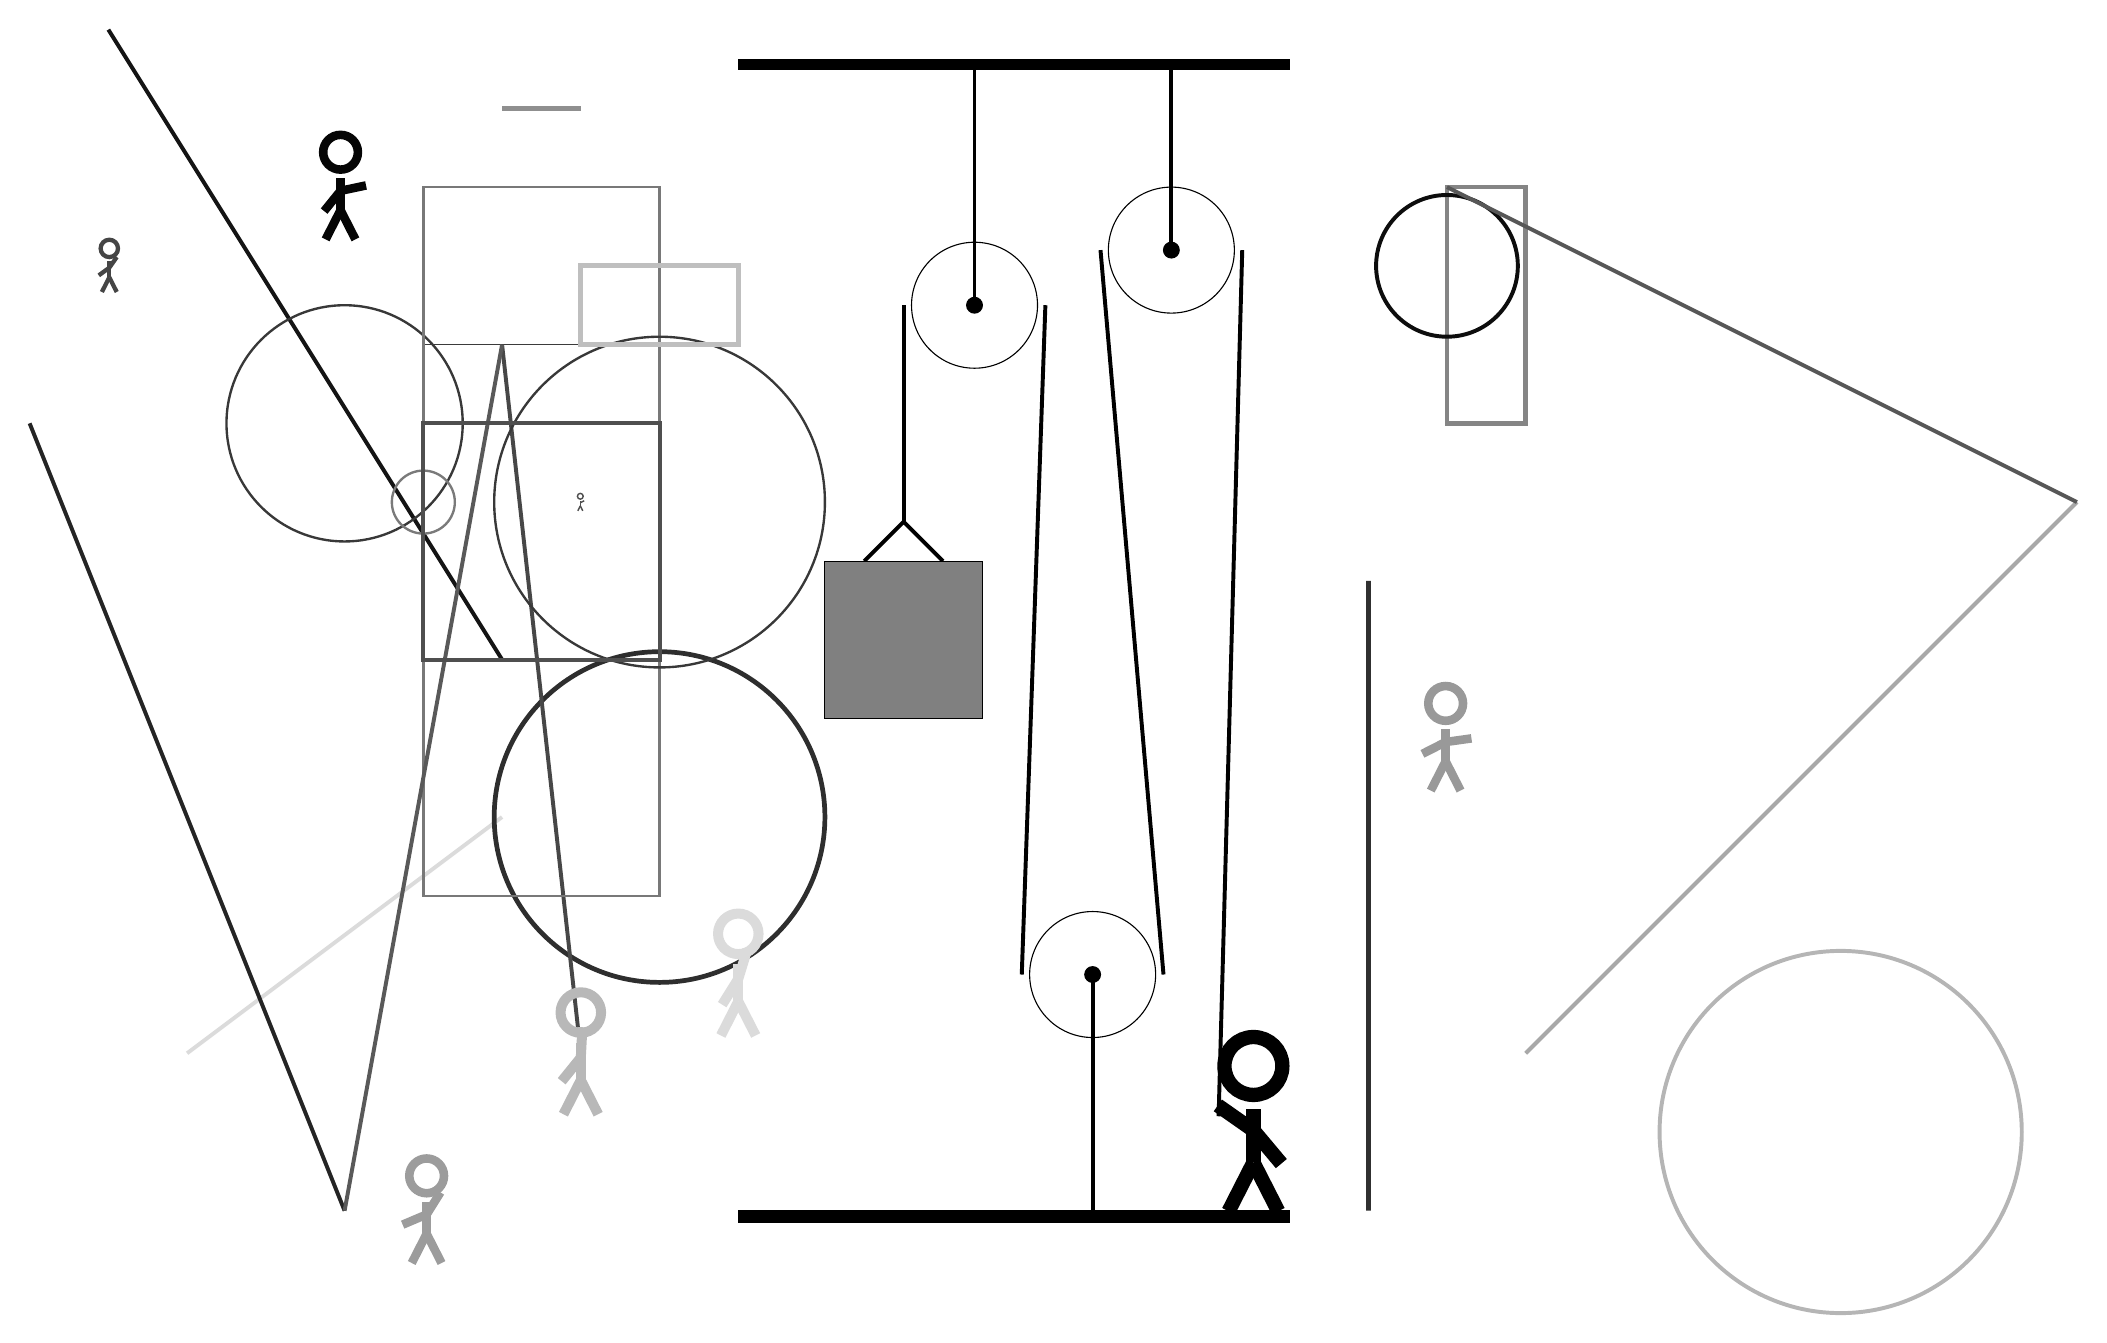
\begin{tikzpicture}
			%%%%% START %%%%%
			
			\draw[fill=black] (-2, 11.5) rectangle (5, 11.625);
			
			\draw (1, 8.5) circle (0.8);
			\draw[fill=black] (1, 8.5) circle (0.1);
			\draw[line width=0.5mm]  (1, 11.5) -- (1, 8.5);
			
			\draw[fill=white](2.5, 0.0) circle (0.8);
			\draw[fill=black] (2.5, 0.0) circle (0.1);
			\draw[line width=0.5mm]  (2.5, -3) -- (2.5, 0.0);
			
			\draw[line width=0.5mm, color=black!14](-5, 2) -- (-9, -1);
			
			\draw[line width=0.5mm, color=black!92](-5, 4) -- (-10, 12);
			\draw[line width=0.7mm, color=black!44] (-4, 11) rectangle (-5, 11);
			\draw [line width=0.5mm, color=black!29](12, -2) circle (2.3);
			
			\node[line width=0.3mm, color=black!39] at (-6, -3) {\Strichmaxerl[6][23][58]};
			
			\draw[line width=0.6mm, color=black!81] (6, -3) rectangle (6, 5);
			\draw[line width=0.5mm, color=black!34](8, -1) -- (15, 6);
			\draw [line width=0.6mm, color=black!82](-3, 2) circle (2.1);
			\draw [line width=0.3mm, color=black!78](-7, 7) circle (1.5);
			
			\draw[line width=0.6mm, color=black!48] (7, 10) rectangle (8, 7);
			\draw [line width=0.5mm, color=black!95](7, 9) circle (0.9);
			\draw[line width=0.2mm, color=black!77] (-3, 7) rectangle (-6, 8);
			\draw[line width=0.5mm, color=black!86](-7, -3) -- (-11, 7);
			\node[line width=0.6mm, color=black!98] at (-7, 10) {\Strichmaxerl[6][51][12]};
			\draw [line width=0.6mm, color=black!36](9, 9) circle (0.0);
			\node[line width=0.6mm, color=black!14] at (-2, 0) {\Strichmaxerl[7][58][73]};
			\draw [line width=0.3mm, color=black!52](-6, 6) circle (0.4);
			\node[line width=0.7mm, color=black!40] at (7, 3) {\Strichmaxerl[6][27][8]};
			\draw[line width=0.5mm, color=black!72](-4, -1) -- (-5, 8);
			\draw[line width=0.3mm, color=black!53] (-3, 1) rectangle (-6, 10);
			\node[line width=0.3mm, color=black!28] at (-4, -1) {\Strichmaxerl[7][51][87]};
			
			\draw [line width=0.3mm, color=black!78](-3, 6) circle (2.1);
			
			\draw[line width=0.5mm, color=black!65](-7, -3) -- (-5, 8);
			\draw[line width=0.5mm, color=black!69] (-3, 4) rectangle (-6, 7);
			\node[line width=0.5mm, color=black!69] at (-4, 6) {\Strichmaxerl[1][90][26]};
			
			\draw[line width=0.5mm, color=black!66](7, 10) -- (15, 6);
			\node[line width=0.2mm, color=black!73] at (-10, 9) {\Strichmaxerl[3][36][55]};
			\draw[line width=0.6mm, color=black!25] (-4, 9) rectangle (-2, 8);
			
			\draw[fill=white](3.5, 9.2) circle (0.8);
			\draw[fill=black] (3.5, 9.2) circle (0.1);
			\draw[line width=0.5mm] (3.5, 11.5) -- (3.5, 9.2);
			
			\draw[line width=0.5mm] (-0.4, 5.25) -- (0.1, 5.75) -- (0.6, 5.25);
			\draw[fill=black!50] (-0.9, 5.25) rectangle (1.1, 3.25);
			
			\draw[line width=0.5mm] (0.1, 8.5) -- (0.1, 5.75);
			\centerarc[line width=0.5mm](1, 8.5)(0:180:0.9);
			\draw[line width=0.5mm](1.9, 8.5) -- (1.6, 0.0);
			\centerarc[line width=0.5mm](2.5, 0.0)(180:360:0.9);
			\draw[line width=0.5mm](3.4, 0.0) -- (2.6, 9.2);
			\centerarc[line width=0.5mm](3.5, 9.2)(0:180:0.9);
			\draw[line width=0.5mm](4.4, 9.2) -- (4.1, -1.8);
			
			\node at (4.5, -1.9) {\Strichmaxerl[10][-35][-50]};
			
			\draw[fill=black] (-2, -3) rectangle (5, -3.15);
			
			%%%%% END %%%%%
		\end{tikzpicture}
	\end{figure}	
\end{document}